\documentclass{standalone}
% Adjust page margins
\usepackage{tikz}
\usetikzlibrary{decorations.markings,arrows.meta}
\usepackage[]{lscape}
\usepackage{amsmath} % For \text{}
\begin{document}
	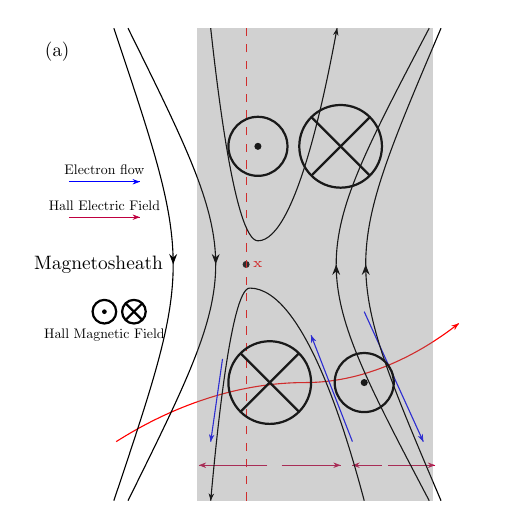
\begin{tikzpicture}[scale=1.5]
		\tikzset{
			thin/.style={line width=0.4pt}, % default thin line
			thick/.style={line width=0.8pt}, % thicker line
			ultra thick/.style={line width=1.5pt} % very thick line
		}
			% Define a generic decoration for an arrow in the middle of the path
			
		\tikzset{
			arrow in middle/.style 2 args={
				decoration={markings,
					mark=at position 0.5 with {\arrow[line width=1pt, scale=0.5]{#1}}},
				postaction={decorate},
				draw=#2
			}
		}
		Define a decoration for a Stealth arrow at the end of the path
		\tikzset{
			arrow at end/.style={
				postaction={decorate},
				decoration={markings,
					mark=at position 1 with {\arrow[line width=0.5pt, scale=0.5]{Stealth}}}
			}
		}
		
			% Draw the center X point
			\fill[ultra thin] (0, 0) circle (0.03);
			\node[red] at (0.1, 0) {\tiny x};
			
			% Draw the central dashed line
			\draw[red, dashed] (0, -2) -- (0,2);
			\draw[thin, draw=purple, arrow at end] (0.18, -1.7) -- (-0.4, -1.7);
			\draw[thin, draw=purple, arrow at end] (0.3, -1.7) -- (0.8, -1.7);
			\draw[thin, draw=purple, arrow at end] (1.15, -1.7) -- (0.9, -1.7);
			\draw[thin, draw=purple, arrow at end] (1.2, -1.7) -- (1.6, -1.7);
			
			\draw[thin, red,arrow at end] (-1.1, -1.5) parabola bend (0.5, -1.0) (1.8, -0.5);
			
			\draw[thin,blue,arrow at end] (-0.2, -0.8)--(-0.3, -1.5) ;
			\draw[thin,blue,arrow at end] (0.9, -1.5)-- (0.55, -0.6);
			\draw[thin,blue,arrow at end] (1.0, -0.4)-- (1.5, -1.5);
		
		    
		    % Add a vertical rectangle
		    \draw[ultra thin, draw=none] (-1.8, 2) rectangle (1, -2);
		    \fill[gray, opacity=0.2] (-0.42, 2) rectangle (1.58, -2);

				%left parabolas
			\draw[thin, arrow in middle={Stealth}{black}] (-1, 2) .. controls (-0.01, 0) .. (-1, -2);
			%\draw[thin, arrow in middle={Stealth}{black}] (-1.1, 2) .. controls (-0.5, 0) .. (-1.1, -2);
			\draw[thin, arrow in middle={Stealth}{black}] (-1.12, 2) .. controls (-0.45, 0) .. (-1.12, -2);
		% Right parabolas
		\draw[thin, arrow in middle={Stealth}{black}] (1.55, -2) .. controls (0.5, 0) .. (1.55, 2);
		%\draw[thin, arrow in middle={Stealth}{black}] (1.6, -2) .. controls (1.2, 0) .. (1.6, 2);
		\draw[thin, arrow in middle={Stealth}{black}] (1.65, -2) .. controls (0.8, 0) .. (1.65, 2);
		
		% Add black parabolas opening outward with arrows at the top
		\draw[thin, arrow at end] (-0.3, 2) parabola bend (0.1, 0.2) (0.77, 2);
		\draw[thin, arrow at end] (1.0, -2) parabola bend (0.03, -0.2) (-0.3, -2);
		
		
		
		\definecolor{darkgreen}{rgb}{0.0, 0.5, 0.0}


	% bottom-left circle
	\def\centerx{0.2}
	\def\centery{-1}
	\def\radius{0.35}
	
	%bottom -right circle 
	\draw[thick,black] (1, -1) circle (0.25);\fill[black] (1, -1) circle (0.03);
	
	% Draw the circle
	\draw[thick,black] (\centerx, \centery) circle (\radius);
	
	% Define the angle in degrees
	\def\angle{45}
	
	% Calculate the coordinates using trigonometric functions
	\pgfmathsetmacro{\xone}{\centerx + \radius * cos(\angle)}
	\pgfmathsetmacro{\yone}{\centery + \radius * sin(\angle)}
	\pgfmathsetmacro{\xtwo}{\centerx - \radius * cos(\angle)}
	\pgfmathsetmacro{\ytwo}{\centery - \radius * sin(\angle)}
	
	\pgfmathsetmacro{\xthree}{\centerx + \radius * cos(135)}
	\pgfmathsetmacro{\ythree}{\centery + \radius * sin(135)}
	\pgfmathsetmacro{\xfour}{\centerx - \radius * cos(135)}
	\pgfmathsetmacro{\yfour}{\centery - \radius * sin(135)}

	% Draw the first diagonal
	\draw[thick,black] (\xone, \yone) -- (\xtwo, \ytwo);	
	% Draw the second diagonal
	\draw[thick,black] (\xthree, \ythree) -- (\xfour, \yfour);


	% top-right-circle
	\def\centerxl{0.8}
	\def\centeryl{1}
	\def\radiusl{0.35}
	
	%top -left circle 
	\draw[thick,black] (0.1, 1) circle (0.25);\fill[black] (0.1, 1) circle (0.03);
	\draw[thick,black] (\centerxl, \centeryl) circle (\radiusl);
	
	% Define the angle in degrees
	\def\angle{45}
	
	% Calculate the coordinates using trigonometric functions
	\pgfmathsetmacro{\xone}{\centerxl + \radiusl * cos(\angle)}
	\pgfmathsetmacro{\yone}{\centeryl + \radiusl * sin(\angle)}
	\pgfmathsetmacro{\xtwo}{\centerxl - \radiusl * cos(\angle)}
	\pgfmathsetmacro{\ytwo}{\centeryl - \radiusl * sin(\angle)}
	
	\pgfmathsetmacro{\xthree}{\centerxl + \radiusl * cos(135)}
	\pgfmathsetmacro{\ythree}{\centeryl + \radiusl * sin(135)}
	\pgfmathsetmacro{\xfour}{\centerxl - \radiusl * cos(135)}
	\pgfmathsetmacro{\yfour}{\centeryl - \radiusl * sin(135)}
	% Draw the first diagonal
	\draw[thick,black] (\xone, \yone) -- (\xtwo, \ytwo);
	% Draw the second diagonal
	\draw[thick,black] (\xthree, \ythree) -- (\xfour, \yfour);
	
	%\draw[line width=0.6pt, red,arrow at end] (2, -1.7) .. controls (1.5, -1.3)and (0, -1.2)  .. (-1, -1);
	
% Draw the rectangle (for reference)
\draw[ultra thin, draw=none] (-1, 2) rectangle (2, -2);
\fill[gray, opacity=0.2] (-0.42, 2) rectangle (1.58, -2);


% Add smaller text label
\node[scale=0.7] at (-1.25, 0) {Magnetosheath} ;
\node[thick,scale=0.7] at (-1.6, 1.8) {(a)};
%bottom -right circle 
\draw[thick,black] (-1.2, -0.4) circle (0.1);\fill[black] (-1.2, -0.4) circle (0.02);
	% sph-right-circle
\node[scale=0.5] at (-1.2, -0.6) {Hall Magnetic Field};
\draw[thin,purple,arrow at end] (-1.5, 0.4) -- (-0.9,0.4);
\node[scale=0.5] at (-1.2, 0.5) {Hall Electric Field};
\draw[thin,blue,arrow at end] (-1.5, 0.7) -- (-0.9,0.7);
\node[scale=0.5] at (-1.2, 0.8) {Electron flow};
			
			% sph-right-circle
			\def\centerxr{-0.95}
			\def\centeryr{-0.4}
			\def\radiusr{0.1}
			
			%top -left circle 
			\draw[thick,black] (\centerxr, \centeryr) circle (\radiusr);
			
			% Define the angle in degrees
			\def\angle{45}
			
			% Calculate the coordinates using trigonometric functions
			\pgfmathsetmacro{\xone}{\centerxr + \radiusr * cos(\angle)}
			\pgfmathsetmacro{\yone}{\centeryr + \radiusr * sin(\angle)}
			\pgfmathsetmacro{\xtwo}{\centerxr - \radiusr * cos(\angle)}
			\pgfmathsetmacro{\ytwo}{\centeryr - \radiusr * sin(\angle)}
			
			\pgfmathsetmacro{\xthree}{\centerxr + \radiusr * cos(135)}
			\pgfmathsetmacro{\ythree}{\centeryr + \radiusr * sin(135)}
			\pgfmathsetmacro{\xfour}{\centerxr - \radiusr * cos(135)}
			\pgfmathsetmacro{\yfour}{\centeryr - \radiusr * sin(135)}
			% Draw the first diagonal
		\draw[thick,black] (\xone, \yone) -- (\xtwo, \ytwo);
		% Draw the second diagonal
		\draw[thick,black] (\xthree, \ythree) -- (\xfour, \yfour);
			
	\end{tikzpicture}
	
		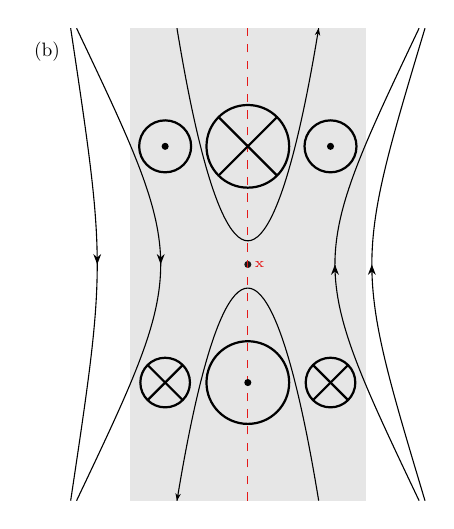
\begin{tikzpicture}[scale=1.5]
		% Define a generic decoration for an arrow in the middle of the path
		\tikzset{
			arrow in middle/.style 2 args={
				decoration={markings,
					mark=at position 0.5 with {\arrow[line width=1pt, scale=0.5]{#1}}},
				postaction={decorate},
				draw=#2
			}
		}
		Define a decoration for a Stealth arrow at the end of the path
		\tikzset{
			arrow at end/.style={
				postaction={decorate},
				decoration={markings,
					mark=at position 1 with {\arrow[line width=0.5pt, scale=0.5]{Stealth}}}
			}
		}
		
		% Draw the center X point
		\fill[ultra thin] (0, 0) circle (0.03);
		\node[red] at (0.1, 0) {\tiny x};
		
		% Draw the central dashed line
		\draw[red, dashed] (0, -2) -- (0,2);
	

		

		
		% Add a vertical rectangle
		 Draw the rectangle (for reference)
		\draw[ultra thin, draw=none] (-1.8, 2) rectangle (0.8, -2);
		\fill[gray, opacity=0.2] (-1, 2) rectangle (1, -2);
		
		%left parabolas
		\draw[thin, arrow in middle={Stealth}{black}] (-1.5, 2) .. controls (-1.2, 0) .. (-1.5, -2);
		\draw[thin, arrow in middle={Stealth}{black}] (-1.45, 2) .. controls (-0.5, 0) .. (-1.45, -2);
		
		%Right parabolas
		\draw[thin, arrow in middle={Stealth}{black}] (1.5, -2) .. controls (0.9, 0) .. (1.5, 2);
		\draw[thin, arrow in middle={Stealth}{black}] (1.45, -2) .. controls (0.5, 0) .. (1.45, 2);
	
		
		% Add black parabolas opening outward with arrows at the top
		\draw[thin, arrow at end] (-0.6, 2) parabola bend (0, 0.2) (0.6, 2);
		\draw[thin, arrow at end] (0.6, -2) parabola bend (0, -0.2) (-0.6, -2);
		
		
		
		\definecolor{darkgreen}{rgb}{0.0, 0.5, 0.0}
		% Add green vertical parabolas on either side below
		%\draw[thin, darkgreen, arrow at end] (-0.4, -2) .. controls (0.18, 0.3) .. (0.7, -2);
		%\draw[thin, darkgreen, arrow at end] (1.3, -2) .. controls (0.75, 0.3) .. (0.8, -2);
		
		
		% top-center circle
		\def\centerx{0}
		\def\centery{1}
		\def\radius{0.35}
		
		%top -right,left circle 
		\draw[thick,black] (0.7, 1) circle (0.22);\fill[black] (0.7, 1) circle (0.03);
		\draw[thick,black] (-0.7, 1) circle (0.22);\fill[black] (-0.7,1) circle (0.03);
		\draw[thick,black] (\centerx, \centery) circle (\radius);
		
		% Define the angle in degrees
		\def\angle{45}
		
		% Calculate the coordinates using trigonometric functions
		\pgfmathsetmacro{\xone}{\centerx + \radius * cos(\angle)}
		\pgfmathsetmacro{\yone}{\centery + \radius * sin(\angle)}
		\pgfmathsetmacro{\xtwo}{\centerx - \radius * cos(\angle)}
		\pgfmathsetmacro{\ytwo}{\centery - \radius * sin(\angle)}
		
		\pgfmathsetmacro{\xthree}{\centerx + \radius * cos(135)}
		\pgfmathsetmacro{\ythree}{\centery + \radius * sin(135)}
		\pgfmathsetmacro{\xfour}{\centerx - \radius * cos(135)}
		\pgfmathsetmacro{\yfour}{\centery - \radius * sin(135)}
		
		% Draw the first diagonal
		\draw[thick,black] (\xone, \yone) -- (\xtwo, \ytwo);	
		% Draw the second diagonal
		\draw[thick,black] (\xthree, \ythree) -- (\xfour, \yfour);
		
		
		% bottom-right left-circle
		\def\centerxl{0.7}
		\def\centeryl{-1}
		\def\radiusl{0.21}
		
		\def\centerxr{-0.7}
		\def\centeryr{-1}
		\def\radiusr{0.21}
		
		%  bottom - center circle 
		\draw[thick,black] (0, -1) circle (0.35);\fill[black] (0, -1) circle (0.03);
		\draw[thick,black] (\centerxl, \centeryl) circle (\radiusl);
		
		% Define the angle in degrees
		\def\angle{45}
		
		% Calculate the coordinates using trigonometric functions
		\pgfmathsetmacro{\xone}{\centerxl + \radiusl * cos(\angle)}
		\pgfmathsetmacro{\yone}{\centeryl + \radiusl * sin(\angle)}
		\pgfmathsetmacro{\xtwo}{\centerxl - \radiusl * cos(\angle)}
		\pgfmathsetmacro{\ytwo}{\centeryl - \radiusl * sin(\angle)}
		
		\pgfmathsetmacro{\xthree}{\centerxl + \radiusl * cos(135)}
		\pgfmathsetmacro{\ythree}{\centeryl + \radiusl * sin(135)}
		\pgfmathsetmacro{\xfour}{\centerxl - \radiusl * cos(135)}
		\pgfmathsetmacro{\yfour}{\centeryl - \radiusl * sin(135)}
		% Draw the first diagonal
		\draw[thick,black] (\xone, \yone) -- (\xtwo, \ytwo);
		% Draw the second diagonal
		\draw[thick,black] (\xthree, \ythree) -- (\xfour, \yfour);
		
	
	
		%top -left circle 
		\draw[thick,black] (\centerxr, \centeryr) circle (\radiusr);
		
		% Define the angle in degrees
		\def\angle{45}
		
		% Calculate the coordinates using trigonometric functions
		\pgfmathsetmacro{\xone}{\centerxr + \radiusr * cos(\angle)}
		\pgfmathsetmacro{\yone}{\centeryr + \radiusr * sin(\angle)}
		\pgfmathsetmacro{\xtwo}{\centerxr - \radiusr * cos(\angle)}
		\pgfmathsetmacro{\ytwo}{\centeryr - \radiusr * sin(\angle)}
		
		\pgfmathsetmacro{\xthree}{\centerxr + \radiusr * cos(135)}
		\pgfmathsetmacro{\ythree}{\centeryr + \radiusr * sin(135)}
		\pgfmathsetmacro{\xfour}{\centerxr - \radiusr * cos(135)}
		\pgfmathsetmacro{\yfour}{\centeryr - \radiusr * sin(135)}
		% Draw the first diagonal
		\draw[thick,black] (\xone, \yone) -- (\xtwo, \ytwo);
		% Draw the second diagonal
		\draw[thick,black] (\xthree, \ythree) -- (\xfour, \yfour);
		\node[thick,scale=0.7] at (-1.7, 1.8) {(b)};
	\end{tikzpicture}
	
	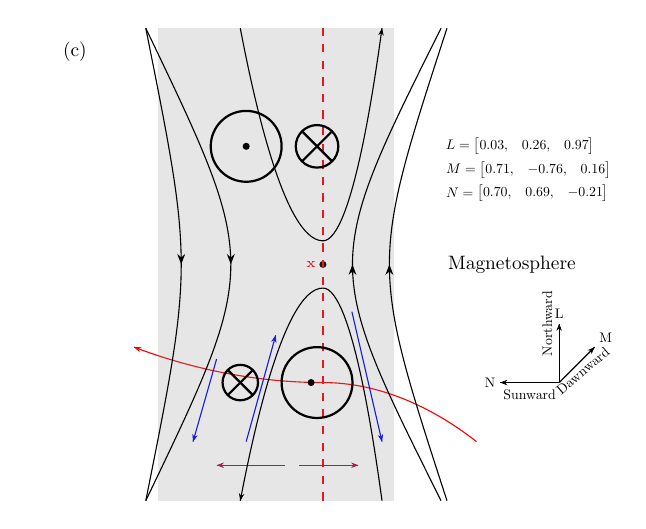
\begin{tikzpicture}[scale=1.5]
	% Define a generic decoration for an arrow in the middle of the path
	\tikzset{
		arrow in middle/.style 2 args={
			decoration={markings,
				mark=at position 0.5 with {\arrow[line width=1pt, scale=0.5]{#1}}},
			postaction={decorate},
			draw=#2
		}
	}
	Define a decoration for a Stealth arrow at the end of the path
	\tikzset{
		arrow at end/.style={
			postaction={decorate},
			decoration={markings,
				mark=at position 1 with {\arrow[line width=0.5pt, scale=0.5]{Stealth}}}
		}
	}
	
	% Draw the center X point
	\fill[ultra thin] (0.5, 0) circle (0.03);
	\node[red] at (0.4, 0) {\tiny x};
	
	% Draw the central dashed line
	\draw[red, dashed] (0.5, -2) -- (0.5,2);
	\draw[thin, draw=purple, arrow at end] (0.18, -1.7) -- (-0.4, -1.7);
	\draw[thin, draw=purple, arrow at end] (0.3, -1.7) -- (0.8, -1.7);
	
	
	\draw[thin, red,arrow at end] (1.8, -1.5) parabola bend (0.5, -1.0) (-1.1, -.7);
	
	\draw[thin,blue,arrow at end] (-0.4, -0.8)--(-0.6, -1.5) ;
	\draw[thin,blue,arrow at end] (-0.15, -1.5)-- (0.1, -0.6);
	\draw[thin,blue,arrow at end] (0.745, -0.4)-- (1, -1.5);


		% Draw the rectangle (for reference)
	\draw[ultra thin, draw=none] (-2, 2) rectangle (3, -2);
	\fill[gray, opacity=0.2] (-0.9, 2) rectangle (1.1, -2);
	
	%left parabolas
	\draw[thin, arrow in middle={Stealth}{black}] (-1, 2) .. controls (-0.04, 0) .. (-1, -2);
	
	\draw[thin, arrow in middle={Stealth}{black}] (-1, 2) .. controls (-0.6, 0) .. (-1, -2);
	% Right parabolas
	\draw[thin, arrow in middle={Stealth}{black}] (1.5, -2) .. controls (0.5, 0) .. (1.5, 2);

	\draw[thin, arrow in middle={Stealth}{black}] (1.55, -2) .. controls (0.9, 0) .. (1.55, 2);
	
	% Add black parabolas opening outward with arrows at the top
	\draw[thin, arrow at end] (-0.2, 2) parabola bend (0.5, 0.2) (1, 2);
	\draw[thin, arrow at end] (1, -2) parabola bend (0.5, -0.2) (-0.2, -2);
	

	\definecolor{darkgreen}{rgb}{0.0, 0.5, 0.0}
	% Add green vertical parabolas on either side below
	%\draw[thin, darkgreen, arrow at end] (-0.4, -2) .. controls (0.18, 0.3) .. (0.7, -2);
	%\draw[thin, darkgreen, arrow at end] (1.3, -2) .. controls (0.75, 0.3) .. (0.8, -2);
	
	
	% bottom-left circle
	\def\centerx{-0.2}
	\def\centery{-1}
	\def\radius{0.15}
	
	%bottom -right circle 
	\draw[thick,black] (0.45, -1) circle (0.3);\fill[black] (0.4, -1) circle (0.03);
	
	% Draw the circle
	\draw[thick,black] (\centerx, \centery) circle (\radius);
		% top-right-circle
	\def\centerxl{0.45}
	\def\centeryl{1}
	\def\radiusl{0.18}
	
	%top -left circle 
	\draw[thick,black] (-0.15, 1) circle (0.3);\fill[black] (-0.15, 1) circle (0.03);
	\draw[thick,black] (\centerxl, \centeryl) circle (\radiusl);
	% Define the angle in degrees
	\def\angle{45}
	
	% Calculate the coordinates using trigonometric functions
	\pgfmathsetmacro{\xone}{\centerx + \radius * cos(\angle)}
	\pgfmathsetmacro{\yone}{\centery + \radius * sin(\angle)}
	\pgfmathsetmacro{\xtwo}{\centerx - \radius * cos(\angle)}
	\pgfmathsetmacro{\ytwo}{\centery - \radius * sin(\angle)}
	
	\pgfmathsetmacro{\xthree}{\centerx + \radius * cos(135)}
	\pgfmathsetmacro{\ythree}{\centery + \radius * sin(135)}
	\pgfmathsetmacro{\xfour}{\centerx - \radius * cos(135)}
	\pgfmathsetmacro{\yfour}{\centery - \radius * sin(135)}
	
	% Draw the first diagonal
	\draw[thick,black] (\xone, \yone) -- (\xtwo, \ytwo);	
	% Draw the second diagonal
	\draw[thick,black] (\xthree, \ythree) -- (\xfour, \yfour);
	
	

	
	% Define the angle in degrees
	\def\angle{45}
	
	% Calculate the coordinates using trigonometric functions
	\pgfmathsetmacro{\xone}{\centerxl + \radiusl * cos(\angle)}
	\pgfmathsetmacro{\yone}{\centeryl + \radiusl * sin(\angle)}
	\pgfmathsetmacro{\xtwo}{\centerxl - \radiusl * cos(\angle)}
	\pgfmathsetmacro{\ytwo}{\centeryl - \radiusl * sin(\angle)}
	
	\pgfmathsetmacro{\xthree}{\centerxl + \radiusl * cos(135)}
	\pgfmathsetmacro{\ythree}{\centeryl + \radiusl * sin(135)}
	\pgfmathsetmacro{\xfour}{\centerxl - \radiusl * cos(135)}
	\pgfmathsetmacro{\yfour}{\centeryl - \radiusl * sin(135)}
	% Draw the first diagonal
	\draw[thick,black] (\xone, \yone) -- (\xtwo, \ytwo);
	% Draw the second diagonal
	\draw[thick,black] (\xthree, \ythree) -- (\xfour, \yfour);
	
	%\draw[line width=0.6pt, red,arrow at end] (2, -1.7) .. controls (1.5, -1.3)and (0, -1.2)  .. (-1, -1);
	

	
	% Add smaller text label
	\node[thick,scale=0.7] at (2.1, 0) {Magnetosphere};
	\node[thick,scale=0.7] at (-1.6, 1.8) {(c)};
	
	
	% Add N, L, M axis labels
	\draw[arrow at end] (2.5, -1) -- (2, -1) node[left, scale=0.5] {N}; % Adjust scale for smaller text
	\draw[arrow at end] (2.5, -1) -- (2.5, -0.5) node[above, scale=0.5] {L};
	\draw[arrow at end] (2.5, -1) -- (2.8, -0.7) node[above right, scale=0.5] {M};
	
	% Add smaller rotated label
	\node[thick,rotate=90, scale=0.5] at (2.4, -0.5) {Northward};
	\node[thick,rotate=0, scale=0.5] at (2.25, -1.1) {Sunward};
	\node[thick,rotate=40, scale=0.5] at (2.7, -0.9) {Dawnward};
	
	% Add matrix to the right of the rectangle
	\node[black,anchor=west, scale=0.5] at (1.5, 1.0) {$
		L = \begin{bmatrix}
			0.03, & 0.26, & 0.97
		\end{bmatrix}
		$};
	\node[thick,anchor=west, scale=0.5] at (1.5, 0.8) {$
		M = \begin{bmatrix}
			0.71, & -0.76, & 0.16
		\end{bmatrix}
		$};
	\node[thick,anchor=west, scale=0.5] at (1.5, 0.6) {$
		N = \begin{bmatrix}
			0.70, & 0.69, & -0.21
		\end{bmatrix}
		$};

\end{tikzpicture}

\end{document}